\documentclass{../ucll-slides}
\usepackage{../pvm}
\usepackage{emerald}
\usepackage[T1]{fontenc}

\title{\cpp: Odi et Amo}
\author{Fr\'ed\'eric Vogels}



\begin{document}

{
  \setbeamercolor{background canvas}{bg=black}
  \ECFJD
  \begin{frame}[plain]
    \begin{center}
      \begin{tikzpicture}[white]
        % \path[use as bounding box] (-5,0) rectangle (5,8);
        \visible<2->{
          \node at (0,8) {
            Please allow me to introduce myself\dots
          };
        }
        \visible<3->{
          \node[anchor=north] (den-bjarne) at (0,7.5) {
            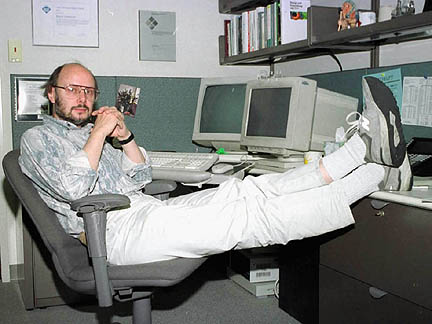
\includegraphics[width=5cm]{BjarneStroustrup.jpg}
          };
        }
        \visible<4->{
          \node[anchor=north] (wealth) at (den-bjarne.south) {
            I'm a man of wealth and taste
          };
        }
        \visible<5->{
          \node[anchor=north] (around) at (wealth.south) {
            I've been around for a long, long year            
          };
        }
        \visible<6->{
          \node[anchor=north] at (around.south) {
            Stole many a man's soul to waste
          };
        }
      \end{tikzpicture}
    \end{center}
  \end{frame}

  \begin{frame}[plain]
    \begin{center}
      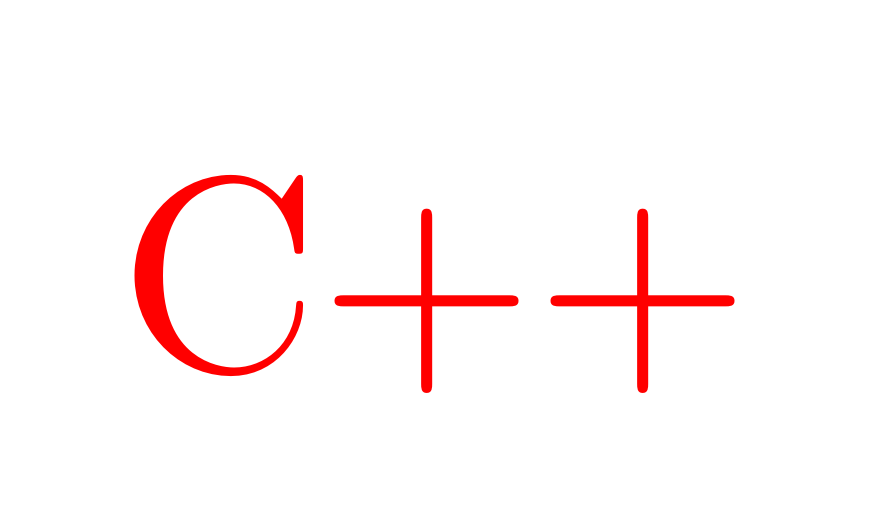
\begin{tikzpicture}[white]
        \node[font=\large] at (0,5) {Bjarne Stroustrup};
        \node at (0,4.5) {presents};
        \node[scale=10,red] at (0,2) {C++};
      \end{tikzpicture}
    \end{center}
  \end{frame}
}


\begin{frame}
  \frametitle{The Good}
  \begin{itemize}
    \item It is a very powerful language
    \item Many very advanced language features
    \item Very efficient, because
          \begin{itemize}
            \item You get full control
            \item Compilers are very, very good at optimising
          \end{itemize}
    \item Exists on any platform
    \item Many existing libraries
    \item Used by many (= lots of helpful resources)
          \begin{itemize}
            \item Most games are made in \cpp\ (efficiency)
            \item Most OSs are written in C/\cpp\ (full control)
          \end{itemize}
  \end{itemize}
\end{frame}

\begin{frame}
  \frametitle{The Bad}
  \begin{itemize}
    \item \cpp\ is a \emph{very} difficult language
          \begin{itemize}
            \item Many rules
            \item Complex rules
            \item Inconsistent rules
          \end{itemize}
    \item Those who like \cpp\ generally do not understand it \\
          (or are masochists)
    \item No safety measures
    \item Mistakes are ``punished'' in the sense that they are not!
          \begin{itemize}
            \item The app merrily goes when mistakes occur
            \item The error only becomes apparent later
          \end{itemize}
    \item Low productivity
          \begin{itemize}
            \item While the code may run fast, it is written slowly
          \end{itemize}
  \end{itemize}
\end{frame}

\begin{frame}
  \frametitle{The Ugly}
  \begin{itemize}
    \item The joys of undefined behaviour
    \item Cryptic compiler errors
    \item \cpp\ = three language for the price of one
          \begin{itemize}
            \item Preprocessor
            \item Templates
            \item ``Regular'' code
          \end{itemize}
    \item IDE support is difficult
  \end{itemize}
\end{frame}


\begin{frame}
  \frametitle{Language Versions and Compilers}
  \begin{columns}
    \begin{column}{5cm}
      \structure{Language versions}
      \begin{itemize}
        \item 1972: C
        \item Cfront: C with classes
        \item 1983: \cpp
        \item 1989: \cpp 2.0
        \item \cpp98
        \item \cpp03
        \item \cpp11
        \item \cpp14
        \item \cpp17
      \end{itemize}
    \end{column}
    \begin{column}{5cm}
      \structure{Compilers}
      \begin{itemize}
        \item MSVC
        \item GCC
        \item Clang
        \item Intel \cpp
        \item HP aCC
        \item Sun/Oracle \cpp
        \item Digital Mars \cpp
        \item Borland (defunct)
        \item Watcom (defunct)
      \end{itemize}
    \end{column}
  \end{columns}
  \begin{center}
    Different compilers support \link{http://en.cppreference.com/w/cpp/compiler_support}{different features}
    of different language versions
  \end{center}
\end{frame}

\begin{frame}
  \frametitle{Unwieldiness}
  \begin{itemize}
    \item Very complex specification
    \item \link{http://www.open-std.org/jtc1/sc22/wg21/docs/papers/2012/n3337.pdf}{Current standard}
          counts 1300+ pages 
    \item Compilers have different interpretations of the standard
    \item Different compilers support different sets of features
    \item Compilers can introduce their own features
    \item Compilers are \emph{very} complex, hence sometimes buggy
  \end{itemize}
\end{frame}

\begin{frame}
  \frametitle{C and \cpp}
  \structure{\cpp's greatest strength is its compatibility with C}
  \begin{itemize}
    \item Familiar syntax
    \item Existing code can be reused
  \end{itemize}
  \vskip5mm
  \structure{\cpp's greatest weakness is its compatibility with C}
  \begin{itemize}
    \item Inherits C's weaknesses
    \item Leads to inconsistencies in language
  \end{itemize}
  \vskip5mm
  \structure{Irony}
  \begin{itemize}
    \item C itself has changed and has introduced incompatibilities
  \end{itemize}
\end{frame}

\begin{frame}
  \frametitle{Efficiency \"Uber Alles!}
  \begin{itemize}
    \item \cpp\ was developped in them good ol' days
          \begin{itemize}
            \item Speed was very important
            \item Memory usage to be kept at a minimum
            \item Many different platforms
          \end{itemize}
    \item Efficiency required during both compilation and execution
    \item Has many consequences on the design of the language
    \item Understanding the reasons makes it easier to understand the language
  \end{itemize}
\end{frame}

\begin{frame}
  \frametitle{Quiz}
  \begin{center}
    \Huge How large is an {\tt int}?
  \end{center}
\end{frame}

\begin{frame}
  \frametitle{Answer}
  \begin{quote}
    There are five standard signed integer types : {\tt signed char}, {\tt short int}, {\tt int}, {\tt long int}, and {\tt long long int}.
    In this list, each type provides at least as much storage as those preceding it in the list.
    [...] Plain {\tt int}s have the natural size suggested by the architecture of the execution environment. \\
    \hfill \link{http://www.open-std.org/jtc1/sc22/wg21/docs/papers/2012/n3337.pdf}{\cpp11 \S 3.9.1/2}
  \end{quote}
  \begin{center}
    \begin{tabular}{lccccc}
      & \rotatebox{90}{\tt char} & \rotatebox{90}{\tt short} & \rotatebox{90}{\tt int} & \rotatebox{90}{\tt long} & \rotatebox{90}{\tt long long} \\
      \toprule
      MSVC (32 bit) & 1 & 2 & 4 & 4 & 8 \\
      MSVC (64 bit) & 1 & 2 & 4 & 4 & 8 \\
      GCC (32 bit)  & 1 & 2 & 4 & 4 & 8 \\
      GCC (64 bit)  & 1 & 2 & 4 & 8 & 8 \\
    \end{tabular}
  \end{center}
\end{frame}

\begin{frame}
  \frametitle{Rationale}
  \begin{itemize}
    \item A 16 bit CPU cannot deal efficiently with 32 bit integers
    \item Java: {\tt int} means ``give me a 32 bit signed integer''
    \item \cpp: {\tt int} means ``give me the largest most efficient integral type on this platform''
    \item Why 4 byte {\tt int}s on 64 bit platforms on MSVC and GCC?
          \begin{itemize}
            \item Probably to keep programs from breaking
          \end{itemize}
  \end{itemize}
\end{frame}

\begin{frame}
  \frametitle{In Practice}
  \begin{itemize}
    \item You will generally use {\tt int}s.
    \item You will generally assume it is 32 bit.
    \item If important, you can use \link{http://en.cppreference.com/w/cpp/language/static_assert}{{\tt static\_assert}}
    \item If size matters, \cpp11 introduced \link{http://en.cppreference.com/w/cpp/types/integer}{{\tt int32\_t}} and other such types
  \end{itemize}
\end{frame}

\begin{frame}
  \frametitle{Quiz}
  \begin{center}
    \Large Assuming {\tt sizeof(int) = 4}, what happens?
    \code[width=5cm]{mult.cpp}
  \end{center}
\end{frame}

\begin{frame}
  \frametitle{Answer}
  \begin{quote}
    If during the evaluation of an expression, the result is not mathematically defined or not in the range of
    representable values for its type, the behavior is undefined. \\
    \hfill \link{http://www.open-std.org/jtc1/sc22/wg21/docs/papers/2012/n3337.pdf}{\cpp11 \S 5/4}
  \end{quote}
  \vskip5mm
  Note that it is not just the result that is undefined but the behaviour of the entire program.
\end{frame}

\begin{frame}
  \frametitle{Rationale}
  \begin{itemize}
    \item Many different representations for negative numbers
    \item If \cpp\ standard makes promises regarding internal representation,
          extra computations would be required on architectures not using that representation
    \item Related example: Java and \link{https://en.wikipedia.org/wiki/Strictfp}{strictfp}
  \end{itemize}
\end{frame}

\begin{frame}
  \frametitle{Java vs \cpp}
  \structure{Java}
  \begin{itemize}
    \item Defines many aspects of VM in detail
    \item Every ``real'' machine must emulate this VM perfectly
    \item If VM disagrees with target machine: inefficient emulation
    \item Luckily, today's architectures are very similar
  \end{itemize}
  \vskip5mm
  \structure{\cpp}
  \begin{itemize}
    \item Developed when architectures were very diverse
    \item \cpp\ is determined to be efficient
    \item \cpp's VM is the intersection of existing machines
    \item Where two architectures differ, \cpp's VM remains vague
    \item VM's specification has many undefined areas
  \end{itemize}
\end{frame}

\begin{frame}
  \frametitle{Quiz}
  \begin{center}
    {\Large What happens?}\vskip1cm
    \code[width=5cm]{array-out-of-bounds.cpp}
  \end{center}
\end{frame}

\begin{frame}
  \frametitle{Answer}
  \begin{quote}
    If both the pointer operand and the result point to elements of the same array object, or one past
    the last element of the array object, the evaluation shall not produce an overflow; otherwise, the behavior is
    undefined.\\
    \hfill \link{http://www.open-std.org/jtc1/sc22/wg21/docs/papers/2012/n3337.pdf}{\cpp11 \S 5.7/6}
  \end{quote}
\end{frame}

\begin{frame}
  \frametitle{Rationale}
  \begin{itemize}
    \item Java checks every array indexing and throws an {\tt ArrayIndexOutOfBounds}
          when you reach out of the array's bounds.
    \item This checking requires extra CPU instructions.
    \item \cpp\ does not check at all. You can use negative indices, or indices that
          go beyond the end of the array, but the resulting behaviour is undefined.
    \item Arrays are not safe, but neither are other containers
  \end{itemize}
\end{frame}

\begin{frame}
  \frametitle{In Practice}
  \begin{itemize}
    \item Generally, you'll assume your code is correct
    \item For safety, you can use assertions (see later)
    \item In debug mode, compilers can add safety measures
  \end{itemize}
\end{frame}

\begin{frame}
  \frametitle{Quiz}
  \begin{center}
    {\Large What happens?}\vskip2cm
    \code[width=8cm]{missing-return.cpp}  
  \end{center}
\end{frame}

\begin{frame}
  \frametitle{Answer}
  \begin{quote}
    Flowing off the end of a function is equivalent to a return with no value; this results in undefined
    behavior in a value-returning function. \\
    \hfill \link{http://www.open-std.org/jtc1/sc22/wg21/docs/papers/2012/n3337.pdf}{\cpp11 \S6.6.3/2}
  \end{quote}
  \begin{itemize}
    \item Compiler is allowed (but not required!) to complain about missing {\tt return}.
    \item If it compiles, running it results in undefined behavior.
  \end{itemize}
\end{frame}

\begin{frame}
  \frametitle{Rationale}
  \begin{itemize}
    \item \cpp\ allows for such complicated constructs
          that it becomes effectively \emph{impossible}
          to determine whether every execution path ends in {\tt return}.
    \item Since it is impossible to determine for \emph{every} program,
          there is no requirement to detect it for \emph{any} program.
  \end{itemize}
\end{frame}

\begin{frame}
  \frametitle{In Practice}
  \begin{itemize}
    \item You \emph{will} encounter this kind of bugs
    \item Using MSVC, debug mode seems to check more
  \end{itemize}
\end{frame}

\begin{frame}
  \frametitle{Quiz}
  \begin{center}
    {\Large What happens?}
    \code[width=8cm]{type-system.cpp}  
  \end{center}
\end{frame}

\begin{frame}
  \frametitle{Answer}
  \begin{quote}
    A prvalue of type {\tt bool} can be converted to a prvalue of type {\tt int}, with {\tt false} becoming zero and {\tt true}
    becoming one. \\
    \hfill \link{http://www.open-std.org/jtc1/sc22/wg21/docs/papers/2012/n3337.pdf}{\cpp11 \S4.5/6}
  \end{quote}
  \begin{itemize}
    \item Passing along {\tt false} where {\tt int[]} is expected is allowed and well defined!
    \item Function will receive null pointer.
  \end{itemize}
\end{frame}

\begin{frame}
  \frametitle{Rationale}
  \begin{itemize}
    \item The type system's main purpose is to allow optimisations
    \item Consider the expression {\tt x + y} 
          \begin{itemize}
            \item If you know the types of both {\tt x} and {\tt y}, you know
                  which assembly instructions to use
            \item If you don't know the types, you need runtime {\tt if}s that check
                  the types at runtime ({\tt int}, {\tt double}, {\tt string}, \dots)
                  and use the appropriate instructions to perform the addition
          \end{itemize}
    \item Type system is rather flexible
    \item Defending against Murphy/Defending against Machiavelli
  \end{itemize}
\end{frame}

\begin{frame}
  \frametitle{Quiz}
  \begin{center}
    {\Large What happens?}
    \code[width=8cm]{uninitialized.cpp}  
  \end{center}
\end{frame}

\begin{frame}
  \frametitle{Answer}
  \begin{itemize}
    \item If you do not initialise variables explicitly, they might contain random values
    \item Some variables are guaranteed to be initialised to zero if you do not specify an initial value yourself
    \item Better be safe than sorry: do not forget to initialise all your variables
  \end{itemize}
\end{frame}

\begin{frame}
  \frametitle{\cpp's Rationale}
  \begin{itemize}
    \item Initialisation takes time
    \item Only those variables that can be initialised for free, are automatically initialised
    \item All other variables have undefined initial values
          \begin{itemize}
            \item Local variables
            \item Object's member variables
            \item Arrays
            \item Allocated memory using {\tt new}
            \item \dots
          \end{itemize}
  \end{itemize}
\end{frame}

\begin{frame}
  \frametitle{Java's Rationale}
  \begin{itemize}
    \item Uninitialised memory = recycled memory
    \item Memory might contain sensitive information (e.g.\ passwords)
    \item JVM zeroes memory to ensure apps cannot access such information
  \end{itemize}
  \code{security.java}
\end{frame}

\begin{frame}
  \frametitle{In Practice}
  \begin{itemize}
    \item You \emph{will} encounter this kind of bugs
    \item MSVC's debug mode uses ``magic numbers''
          \begin{itemize}
            \item {\tt CCCCCCCC}: uninitialised stack memory
            \item {\tt CDCDCDCD}: uninitialised heap memory
            \item {\tt FDFDFDFD}: around heap allocated memory
            \item {\tt FEEEFEEE}: freed memory
          \end{itemize}
    \item If your variables contain one of these values,
          you know you probably are in trouble
  \end{itemize}
\end{frame}

\begin{frame}
  \frametitle{Morality of this Presentation}
  \begin{itemize}
    \item When encountering errors, don't make assumptions
    \item Do check for missing returns
    \item Do check for uninitialised variables
    \item Watch out for special values while debugging
  \end{itemize}
\end{frame}

% Memory safety (can write anywhere)
% Manual memory allocation

\end{document}